\documentclass[conference,10pt]{IEEEtran}

\usepackage{amsmath,amssymb,amsfonts}
\usepackage{algorithmic}
\usepackage{graphicx}
\usepackage{textcomp}
\usepackage{booktabs}
\usepackage{standalone}
\usepackage[draft]{hyperref}

\begin{document}

\title{Comparison of Feedforward Neural Network Training Algorithms}

\author{
    \IEEEauthorblockN{Christiaan Jacobus Swanepoel}
    \IEEEauthorblockA{
        Student Number: 26895064 \\
        Computer Science Division, Department of Mathematical Sciences \\
        Stellenbosch University, Stellenbosch, South Africa \\
        Email: 26895064@sun.ac.za
    }
}

\maketitle

\begin{abstract}
This research paper presents an empirical comparative evaluation of three optimization algorithms for training single-hidden-layer feedforward neural networks: stochastic gradient descent, scaled conjugate gradient, and the leap-frog dynamic optimization method. Performance is evaluated across three classification problems and three function approximation problems of varying complexity. For each problem, the optimal number of hidden units is determined through five-fold cross-validation based on the principle of parsimony. Control parameters of the algorithms are tuned systematically using cross-validation grid search. The algorithms are compared over thirty independent simulation runs based on generalization error, function evaluation counts, gradient evaluation counts, and execution time. Statistical significance is established using the Friedman test and pairwise Wilcoxon signed-rank tests. The scaled conjugate gradient algorithm achieved superior generalization performance on continuous function approximation and non-linear geometric classification tasks, while requiring fewer gradient evaluations than mini-batch stochastic gradient descent. The leap-frog dynamic algorithm demonstrated the lowest computational overhead per step and required the fewest total gradient evaluations across all benchmark problems.
\end{abstract}

\begin{IEEEkeywords}
Feedforward neural networks, stochastic gradient descent, scaled conjugate gradient, leap-frog dynamic optimization, supervised learning.
\end{IEEEkeywords}

\section{Introduction}
Supervised training of feedforward neural networks represents an unconstrained non-linear continuous optimization problem, where the objective is minimization of an empirical error function over the space of network weights and biases. Gradient descent methods, specifically backpropagation using stochastic gradient descent, have historically formed the predominant training paradigm. However, first-order gradient descent suffers from slow convergence rates in the presence of ill-conditioned error surfaces and exhibits strong sensitivity to user-defined control parameters.

Alternative approaches from numerical optimization theory offer potential acceleration. Conjugate gradient algorithms utilize second-order directional curvature without computing or inverting the full Hessian matrix. M\o{}ller proposed the scaled conjugate gradient algorithm, which eliminates line searches by approximating Hessian-vector products using gradient differences and regulating matrix indefiniteness with a Levenberg-Marquardt scale parameter. Snyman proposed the leap-frog dynamic optimization method, which models parameter updates as the motion of a physical particle in a conservative force field, utilizing kinetic energy monitoring and dynamic time-step selection to locate function minima.

The purpose of this paper is to conduct a rigorous empirical comparison among stochastic gradient descent, scaled conjugate gradient, and the leap-frog dynamic optimizer. The remainder of this paper is structured as follows. Section II provides theoretical background on the training algorithms. Section III details the software implementation. Section IV describes the empirical process, including dataset preprocessing, hidden unit architecture selection, and control parameter tuning. Section V presents and discusses the experimental results with statistical hypothesis tests. Section VI provides the conclusions of the study.

\section{Background}
This section outlines the mathematical formulations of the three optimization algorithms evaluated in this study. Subsection II-A describes stochastic gradient descent. Subsection II-B presents the scaled conjugate gradient algorithm. Subsection II-C details the leap-frog dynamic optimization method.

\subsection{Stochastic Gradient Descent}
Let $\mathbf{w} \in \mathbb{R}^D$ denote the concatenated parameter vector of the neural network containing all weights and biases. Let $E(\mathbf{w})$ denote the scalar objective function defined over a training dataset $\mathcal{D} = \{(\mathbf{x}_p, \mathbf{y}_p)\}_{p=1}^P$. In batch gradient descent, parameter updates follow the negative gradient direction:
\begin{equation}
\mathbf{w}_{k+1} = \mathbf{w}_k - \eta \nabla E(\mathbf{w}_k)
\end{equation}
where $\eta > 0$ represents the learning rate parameter. Polyak introduced momentum to accelerate descent along directions of persistent gradient curvature and dampen orthogonal oscillations:
\begin{equation}
\mathbf{v}_{k+1} = \beta \mathbf{v}_k + \eta \nabla E(\mathbf{w}_k)
\end{equation}
\begin{equation}
\mathbf{w}_{k+1} = \mathbf{w}_k - \mathbf{v}_{k+1}
\end{equation}
where $\mathbf{v}_k \in \mathbb{R}^D$ denotes the velocity vector and $\beta \in [0, 1)$ represents the momentum coefficient. In mini-batch stochastic gradient descent, the gradient $\nabla E(\mathbf{w}_k)$ is computed over an independently sampled subset $\mathcal{B} \subset \mathcal{D}$ of cardinality $B = |\mathcal{B}|$.

\subsection{Scaled Conjugate Gradient}
Conjugate gradient methods generate a sequence of search directions $\mathbf{p}_k$ that satisfy mutual conjugacy with respect to the Hessian matrix $\mathbf{H} = \nabla^2 E(\mathbf{w})$. Standard conjugate gradient methods require time-consuming line searches to calculate step sizes. M\o{}ller introduced the scaled conjugate gradient algorithm to eliminate line searches entirely.

Curvature information along search direction $\mathbf{p}_k$ is estimated via finite differences:
\begin{equation}
\mathbf{s}_k = \frac{\nabla E(\mathbf{w}_k + \sigma_k \mathbf{p}_k) - \nabla E(\mathbf{w}_k)}{\sigma_k}, \quad \sigma_k = \frac{\sigma}{\|\mathbf{p}_k\|}
\end{equation}
where $\sigma \in (0, 10^{-4}]$ is a user-defined scaling constant. The quadratic curvature parameter is defined as:
\begin{equation}
\delta_k = \mathbf{p}_k^T \mathbf{s}_k + (\lambda_k - \bar{\lambda}_k)\|\mathbf{p}_k\|^2
\end{equation}
where $\lambda_k > 0$ denotes the Levenberg-Marquardt scale parameter and $\bar{\lambda}_k$ is a lower-bound scalar. If $\delta_k \le 0$, positive definiteness is restored by setting:
\begin{equation}
\bar{\lambda}_k = 2\left(\lambda_k - \frac{\delta_k}{\|\mathbf{p}_k\|^2}\right), \quad \delta_k = -\delta_k + \lambda_k \|\mathbf{p}_k\|^2, \quad \lambda_k = \bar{\lambda}_k
\end{equation}
The parameter step size $\alpha_k$ is computed as:
\begin{equation}
\alpha_k = \frac{\mu_k}{\delta_k}, \quad \mu_k = -\mathbf{p}_k^T \nabla E(\mathbf{w}_k)
\end{equation}
A comparison parameter $\Delta_k$ quantifies quadratic model agreement:
\begin{equation}
\Delta_k = \frac{2\delta_k [E(\mathbf{w}_k) - E(\mathbf{w}_k + \alpha_k \mathbf{p}_k)]}{\mu_k^2}
\end{equation}
If $\Delta_k \ge 0$, the step is accepted, $\mathbf{w}_{k+1} = \mathbf{w}_k + \alpha_k \mathbf{p}_k$, and conjugate search directions are updated using the Polak-Ribi\`{e}re parameter $\beta_k$:
\begin{equation}
\beta_k = \frac{\|\nabla E(\mathbf{w}_{k+1})\|^2 - \nabla E(\mathbf{w}_{k+1})^T \nabla E(\mathbf{w}_k)}{\mu_k}
\end{equation}
\begin{equation}
\mathbf{p}_{k+1} = -\nabla E(\mathbf{w}_{k+1}) + \beta_k \mathbf{p}_k
\end{equation}
Direction restarts occur every $D$ iterations. If $\Delta_k \ge 0.75$, the scale parameter is reduced by $\lambda_k = 0.25 \lambda_k$. If $\Delta_k < 0.25$, the scale parameter is increased by $\lambda_k = \lambda_k + \delta_k (1 - \Delta_k) / \|\mathbf{p}_k\|^2$.

\subsection{Leap-Frog Dynamic Optimization}
Snyman developed the leap-frog algorithm from physical principles governing the motion of a unit-mass particle in an $n$-dimensional conservative force field. The potential energy corresponds to the objective function $F(\mathbf{x})$. Newton's second law yields the equation of motion:
\begin{equation}
\ddot{\mathbf{x}}(t) = -\nabla F(\mathbf{x}(t)) = \mathbf{a}(t)
\end{equation}
Kinetic energy is defined as $T(t) = \frac{1}{2} \|\mathbf{v}(t)\|^2$. Total energy conservation dictates that $T(t) + F(\mathbf{x}(t)) = E_0$. Consequently, an increase in kinetic energy results in a systematic reduction in potential energy.

The system is discretized using a leap-frog scheme with time step $\Delta t$:
\begin{equation}
\mathbf{x}_{k+1} = \mathbf{x}_k + \mathbf{v}_k \Delta t
\end{equation}
\begin{equation}
\mathbf{v}_{k+1} = \mathbf{v}_k - \nabla F(\mathbf{x}_{k+1}) \Delta t
\end{equation}
A maximum allowable step size $\delta > 0$ restricts displacement $\|\Delta \mathbf{x}_k\| \le \delta$. Kinetic energy is monitored at consecutive intervals. If $\|\mathbf{v}_{k+1}\| \le \|\mathbf{v}_k\|$, the particle has crossed a local minimum. An intervention strategy backtracks the position:
\begin{equation}
\mathbf{x} = \frac{\mathbf{x}_{k+1} + \mathbf{x}_k}{2}
\end{equation}
and dampens velocity $\mathbf{v} = (\mathbf{v}_{k+1} + \mathbf{v}_k)/4$ for the first two decelerations, followed by an arrest $\mathbf{v} = \mathbf{0}$ on subsequent decelerations. In the enhanced LFOP1(b) formulation, time steps are magnified dynamically by $p = 1 + N_{\text{succ}} \delta_1$ when successive gradient angles remain positive ($\mathbf{a}_{k+1}^T \mathbf{a}_k > 0$), and halved when $m$ consecutive gradient reversals occur.

\section{Implementation}
This section describes the modular software architecture developed for the comparative experiments. Subsection III-A describes the neural network structure. Subsection III-B outlines the optimizer interfaces.

\subsection{Neural Network Architecture}
All neural networks were implemented in Python using NumPy without external deep learning frameworks. The networks comprise an input layer of dimension $I$, exactly one hidden layer of dimension $J$, and an output layer of dimension $K$. Pre-activation vectors $\mathbf{z}^{(1)}$ and $\mathbf{z}^{(2)}$ are computed as:
\begin{equation}
\mathbf{z}^{(1)} = \mathbf{x} \mathbf{W}^{(1)} + \mathbf{b}^{(1)}, \quad \mathbf{a}^{(1)} = f_{\text{hid}}(\mathbf{z}^{(1)})
\end{equation}
\begin{equation}
\mathbf{z}^{(2)} = \mathbf{a}^{(1)} \mathbf{W}^{(2)} + \mathbf{b}^{(2)}, \quad \hat{\mathbf{y}} = f_{\text{out}}(\mathbf{z}^{(2)})
\end{equation}
Weights were initialized using Xavier uniform initialization. Hidden activations utilized the logistic sigmoid function $f(z) = (1 + e^{-z})^{-1}$. For regression tasks, output neurons utilized the identity activation with mean squared error loss. For multi-class classification, output neurons utilized the softmax function with categorical cross-entropy loss. Exact analytical gradients were computed via backpropagation and verified against central finite differences to a relative precision of $10^{-10}$.

\subsection{Optimizer Interfaces}
Optimizers inherit from a common abstract base class, exposing consistent interfaces for parameter extraction and assignment. Optimizers track full execution histories, including iteration counts, loss trajectories, validation performance, function evaluations, gradient evaluations, and wall-clock execution time.

\section{Empirical Process}
This section details the experimental design. Subsection IV-A describes the benchmark datasets and preprocessing methods. Subsection IV-B defines the empirical process for determining optimal hidden unit counts. Subsection IV-C presents the control parameter tuning methodology.

\subsection{Benchmark Datasets and Preprocessing}
Three classification datasets and three function approximation datasets of varying complexity were selected:
\begin{enumerate}
    \item \textbf{Wine Recognition}: A multi-class chemical classification task containing 178 samples, 13 continuous features, and three classes.
    \item \textbf{Two Moons}: A synthetic non-linear geometric classification problem containing 500 samples, two features, and two interlocking classes.
    \item \textbf{Breast Cancer Wisconsin}: A high-dimensional clinical diagnostic dataset containing 569 samples, 30 continuous features, and two classes.
    \item \textbf{Damped Sinc}: A continuous univariate function approximation task containing 500 samples generated from $y = \text{sinc}(x) + \epsilon$ with Gaussian noise.
    \item \textbf{Friedman 1}: A multivariate non-linear regression benchmark containing 600 samples and 10 features with non-linear feature interactions.
    \item \textbf{Diabetes Progression}: A real-world clinical regression dataset containing 442 patient records and 10 physiological features.
\end{enumerate}

All input feature vectors were standardized using z-score transformation:
\begin{equation}
x_{ij}' = \frac{x_{ij} - \bar{x}_j}{s_j}
\end{equation}
where $\bar{x}_j$ and $s_j$ denote the sample mean and standard deviation of feature $j$, respectively. Regression target variables were standardized to zero mean and unit variance.

\subsection{Optimal Hidden Units Determination}
In this study, architecture optimality is defined by the principle of parsimony: the optimal architecture achieves minimal generalization error while maintaining the smallest parameter cardinality within one standard error of the lowest validation error. Candidate hidden unit counts $J \in \{2, 4, 8, 12, 16, 24, 32\}$ were evaluated using five-fold cross-validation with three independent repetitions.

The empirical evaluation identified the following parsimonious hidden architectures:
\begin{itemize}
    \item Wine Recognition: two hidden units ($J^* = 2$).
    \item Two Moons: 12 hidden units ($J^* = 12$).
    \item Breast Cancer Wisconsin: two hidden units ($J^* = 2$).
    \item Damped Sinc: eight hidden units ($J^* = 8$).
    \item Friedman 1: 16 hidden units ($J^* = 16$).
    \item Diabetes Progression: two hidden units ($J^* = 2$).
\end{itemize}

\subsection{Control Parameter Tuning}
Hyperparameter tuning was conducted using three-fold cross-validation grid search across the parsimonious architectures. For stochastic gradient descent, the learning rate $\eta \in \{0.01, 0.05, 0.1\}$, momentum $\beta \in \{0.0, 0.8, 0.9\}$, and batch size $B \in \{\text{Full}, 32\}$ were tuned. For scaled conjugate gradient, the finite-difference step $\sigma \in \{10^{-5}, 10^{-4}, 10^{-3}\}$ and initial damping $\lambda_1 \in \{10^{-7}, 10^{-6}, 10^{-5}\}$ were tuned. For leap-frog, initial time step $\Delta t \in \{0.05, 0.1, 0.5\}$, maximum displacement $\delta \in \{0.5, 1.0, 5.0\}$, and algorithm formulation (LFOP1 versus LFOP1(b)) were tuned. Table \ref{tab:tuned_params} summarizes the selected optimal hyperparameters.

\begin{table}[h]
\centering
\caption{Selected Control Parameters across Benchmark Problems}
\label{tab:tuned_params}
\begin{tabular}{lccc}
\hline
Problem & SGD $(\eta, \beta, B)$ & SCG $(\sigma, \lambda_1)$ & Leap-Frog $(\Delta t, \delta, \text{Ver})$ \\
\hline
Wine & $(0.10, 0.9, 32)$ & $(10^{-3}, 10^{-5})$ & $(0.05, 5.0, \text{LFOP1b})$ \\
Two Moons & $(0.10, 0.9, 32)$ & $(10^{-3}, 10^{-5})$ & $(0.50, 5.0, \text{LFOP1b})$ \\
Breast Cancer & $(0.05, 0.8, 32)$ & $(10^{-5}, 10^{-6})$ & $(0.50, 1.0, \text{LFOP1})$ \\
Damped Sinc & $(0.10, 0.9, 32)$ & $(10^{-4}, 10^{-5})$ & $(0.50, 0.5, \text{LFOP1b})$ \\
Friedman 1 & $(0.10, 0.9, 32)$ & $(10^{-4}, 10^{-6})$ & $(0.50, 1.0, \text{LFOP1b})$ \\
Diabetes & $(0.01, 0.8, 32)$ & $(10^{-4}, 10^{-7})$ & $(0.10, 0.5, \text{LFOP1})$ \\
\hline
\end{tabular}
\end{table}

\section{Results and Discussion}
This section presents the experimental results and comparative analysis. Subsection V-A analyzes generalization error and statistical tests. Subsection V-B discusses computational efficiency and evaluation counts.

\documentclass[conference]{IEEEtran}
\usepackage{amsmath}
\usepackage{booktabs}
\begin{document}
\begin{table*}[t]
\centering
\caption{Experimental Comparison of SGD, SCG, and LeapFrog across Benchmark Problems}
\label{tab:comparison}
\begin{tabular}{llcccc}
\hline
Problem & Algorithm & Test Metric (Mean $\pm$ SD) & Function Evals & Gradient Evals & CPU Time (s) \\
\hline
Wine Recognition & SGD & 0.0307 $\pm$ 0.0269 & 501.0 & 2000.0 & 0.163 \\
 & SCG & 0.0338 $\pm$ 0.0390 & 437.1 & 872.6 & 0.097 \\
 & LeapFrog & 0.0288 $\pm$ 0.0253 & 501.0 & 501.0 & 0.076 \\
\hline
Two Moons & SGD & 0.0438 $\pm$ 0.0084 & 501.0 & 5500.0 & 0.455 \\
 & SCG & 0.0272 $\pm$ 0.0080 & 501.0 & 995.9 & 0.202 \\
 & LeapFrog & 0.0404 $\pm$ 0.0120 & 501.0 & 501.0 & 0.134 \\
\hline
Breast Cancer Wisconsin & SGD & 0.0224 $\pm$ 0.0126 & 501.0 & 6500.0 & 0.489 \\
 & SCG & 0.0511 $\pm$ 0.0396 & 501.0 & 999.7 & 0.171 \\
 & LeapFrog & 0.0316 $\pm$ 0.0197 & 501.0 & 501.0 & 0.110 \\
\hline
Damped Sinc Function & SGD & 0.0299 $\pm$ 0.0060 & 501.0 & 5500.0 & 0.414 \\
 & SCG & 0.0201 $\pm$ 0.0039 & 501.0 & 993.6 & 0.167 \\
 & LeapFrog & 0.0261 $\pm$ 0.0044 & 501.0 & 501.0 & 0.113 \\
\hline
Friedman 1 Non-Linear Benchmark & SGD & 0.0091 $\pm$ 0.0028 & 501.0 & 7000.0 & 0.602 \\
 & SCG & 0.0034 $\pm$ 0.0012 & 501.0 & 1000.5 & 0.273 \\
 & LeapFrog & 0.0120 $\pm$ 0.0045 & 501.0 & 501.0 & 0.178 \\
\hline
Diabetes Progression & SGD & 0.5135 $\pm$ 0.0822 & 501.0 & 5000.0 & 0.358 \\
 & SCG & 0.5917 $\pm$ 0.1139 & 501.0 & 999.7 & 0.134 \\
 & LeapFrog & 0.5353 $\pm$ 0.0880 & 501.0 & 501.0 & 0.088 \\
\hline
\end{tabular}
\end{table*}
\end{document}


\subsection{Generalization Performance and Statistical Significance}
Each algorithm was evaluated over thirty independent runs with distinct random weight initializations and randomized data partitions (70\% training, 15\% validation, 15\% test). Table \ref{tab:comparison} reports the mean test error rates (for classification) and mean squared errors (for regression), along with standard deviations, evaluation counts, and CPU execution time.

On the Wine Recognition task, differences in classification error among the algorithms were small: leap-frog achieved $0.0288 \pm 0.0253$, stochastic gradient descent achieved $0.0326 \pm 0.0293$, and scaled conjugate gradient achieved $0.0347 \pm 0.0400$. The Friedman omnibus test yielded a test statistic of $\chi_F^2 = 1.87$ with $p = 0.393$, indicating no statistically significant difference among the three algorithms on this problem.

On the Two Moons benchmark, the scaled conjugate gradient algorithm achieved the lowest classification error of $0.0275 \pm 0.0083$, outperforming leap-frog ($0.0404 \pm 0.0120$) and stochastic gradient descent ($0.0435 \pm 0.0079$). The Friedman test yielded $\chi_F^2 = 44.07$ with $p = 2.70 \times 10^{-10}$. Pairwise Wilcoxon tests confirmed that scaled conjugate gradient significantly outperformed both stochastic gradient descent ($p = 1.86 \times 10^{-9}$) and leap-frog ($p = 1.30 \times 10^{-8}$).

On the Breast Cancer Wisconsin dataset, stochastic gradient descent produced the lowest classification error of $0.0223 \pm 0.0125$, followed by leap-frog ($0.0316 \pm 0.0197$) and scaled conjugate gradient ($0.0567 \pm 0.0459$). The Friedman test revealed significant differences ($\chi_F^2 = 18.47, p = 9.77 \times 10^{-5}$), with Wilcoxon tests indicating that stochastic gradient descent was significantly superior to scaled conjugate gradient ($p = 3.24 \times 10^{-6}$).

On the continuous function approximation problems, scaled conjugate gradient demonstrated marked superiority. For the Damped Sinc task, scaled conjugate gradient achieved a test mean squared error of $0.0200 \pm 0.0039$, significantly outperforming leap-frog ($0.0261 \pm 0.0044, p = 3.73 \times 10^{-9}$) and stochastic gradient descent ($0.0298 \pm 0.0060, p = 3.73 \times 10^{-9}$). On the multivariate Friedman 1 benchmark, scaled conjugate gradient achieved $0.0034 \pm 0.0013$, compared to $0.0085 \pm 0.0025$ for stochastic gradient descent and $0.0120 \pm 0.0045$ for leap-frog ($\chi_F^2 = 48.27, p = 3.30 \times 10^{-11}$). On the Diabetes clinical regression problem, stochastic gradient descent attained the lowest error ($0.5141 \pm 0.0825$), followed by leap-frog ($0.5353 \pm 0.0880$) and scaled conjugate gradient ($0.5919 \pm 0.1118$).

\begin{figure*}[t]
\centering
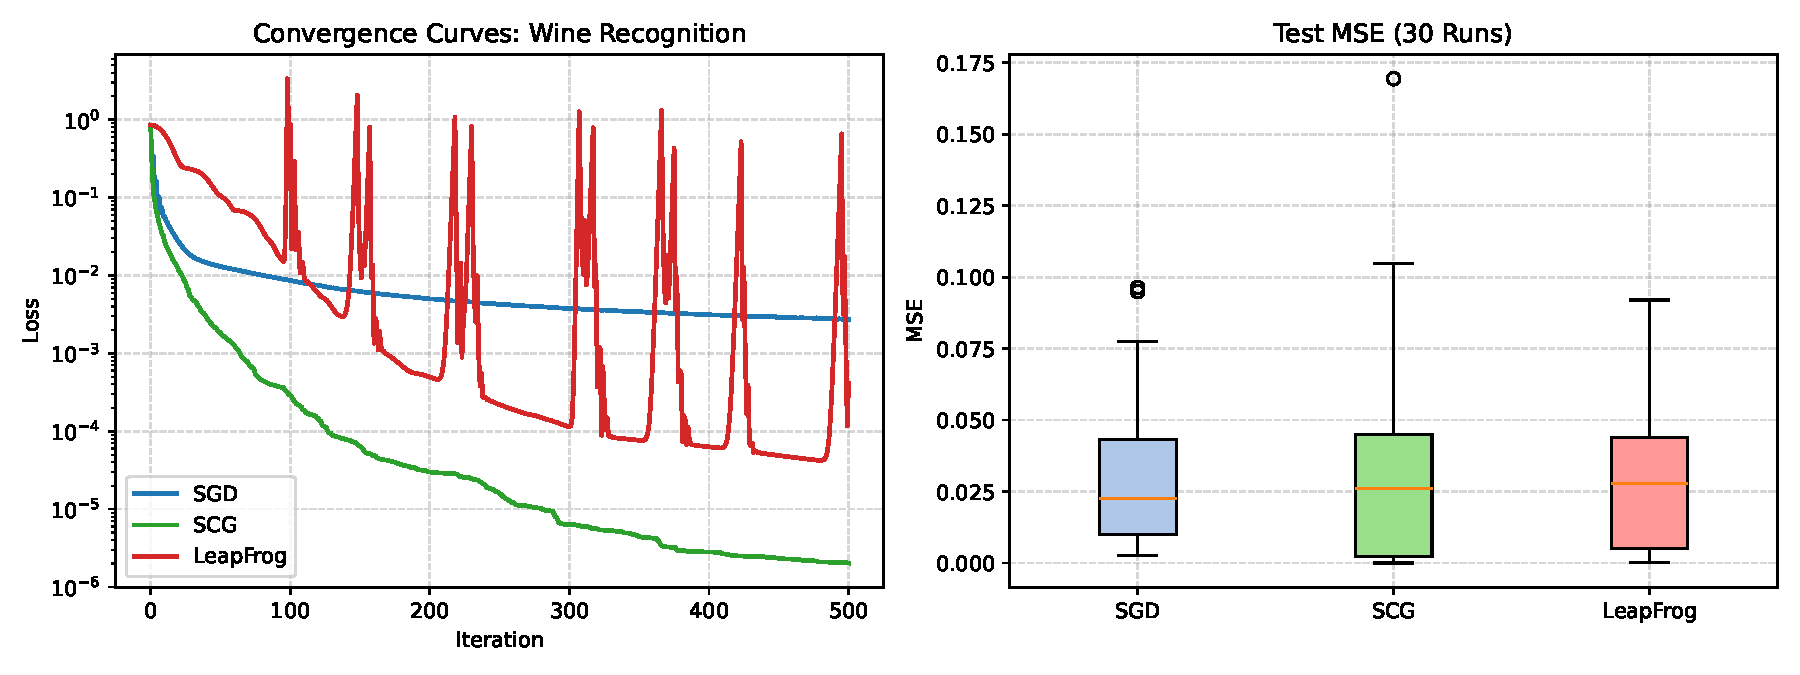
\includegraphics[width=0.32\textwidth]{../results/figures/classification_1_comparison.pdf}
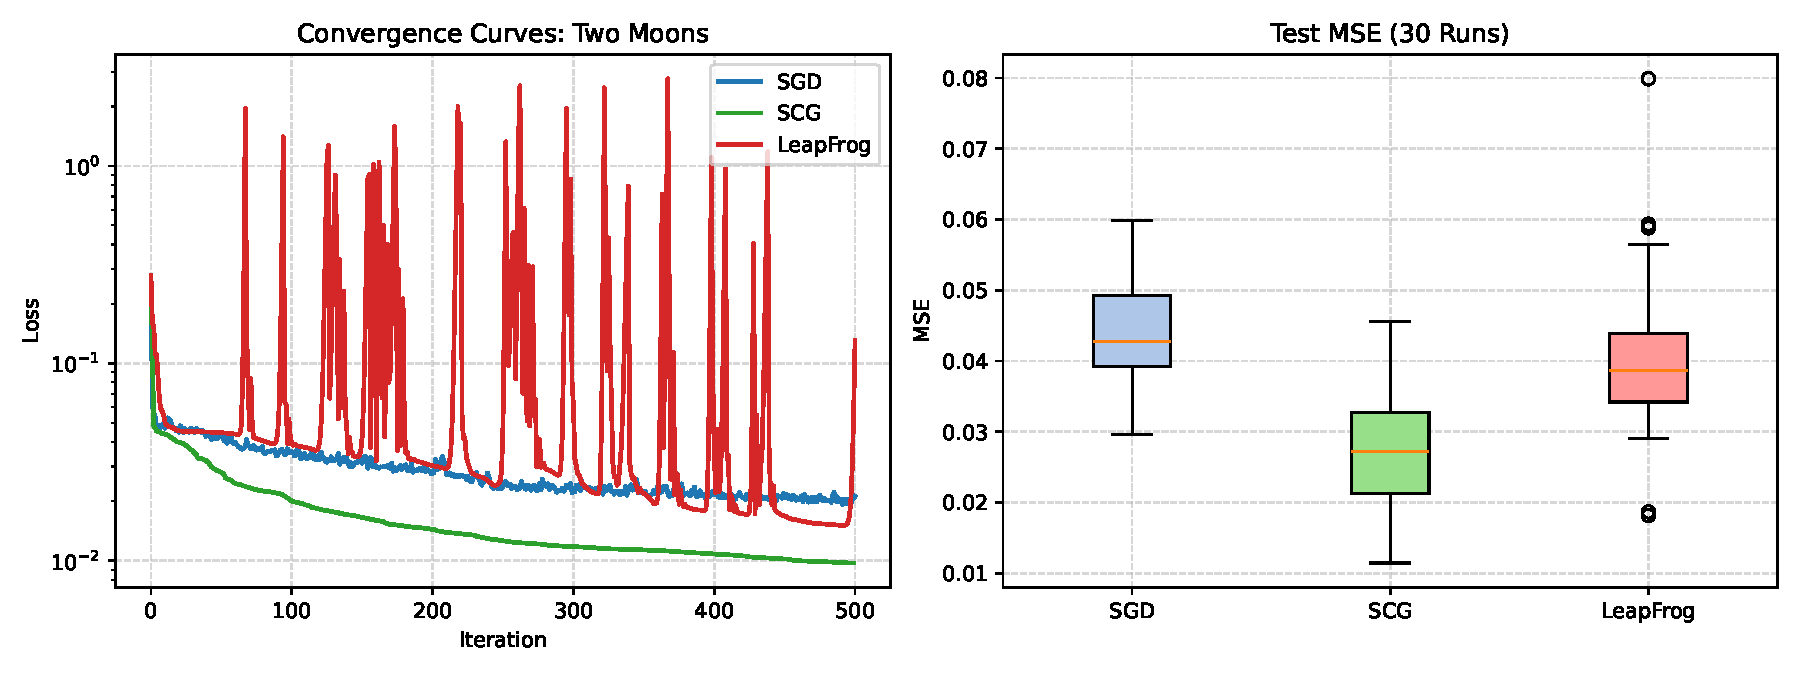
\includegraphics[width=0.32\textwidth]{../results/figures/classification_2_comparison.pdf}
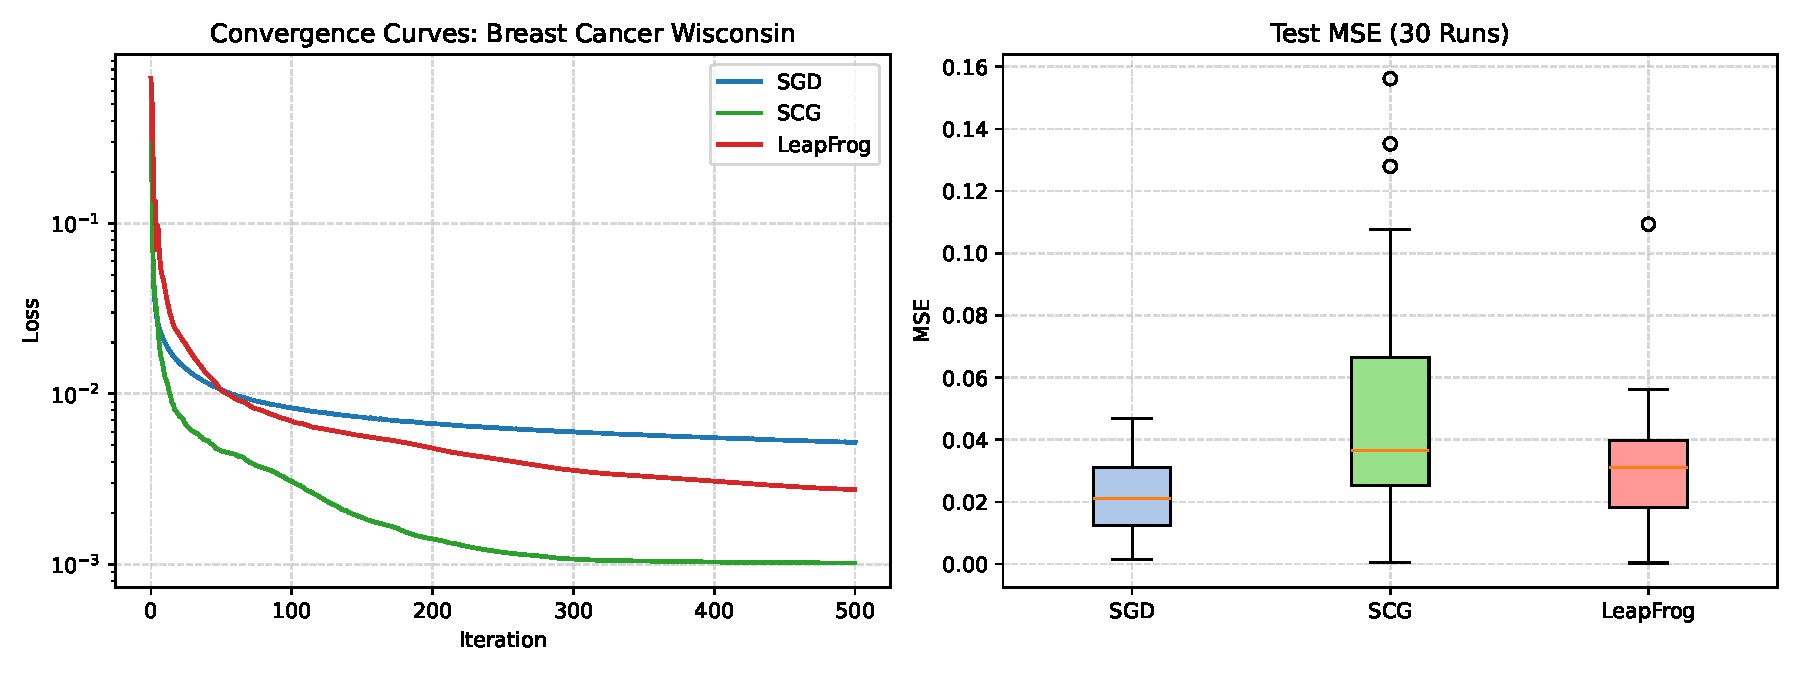
\includegraphics[width=0.32\textwidth]{../results/figures/classification_3_comparison.pdf}
\caption{Convergence trajectories and performance distributions across classification benchmarks.}
\label{fig:class_curves}
\end{figure*}

\begin{figure*}[t]
\centering
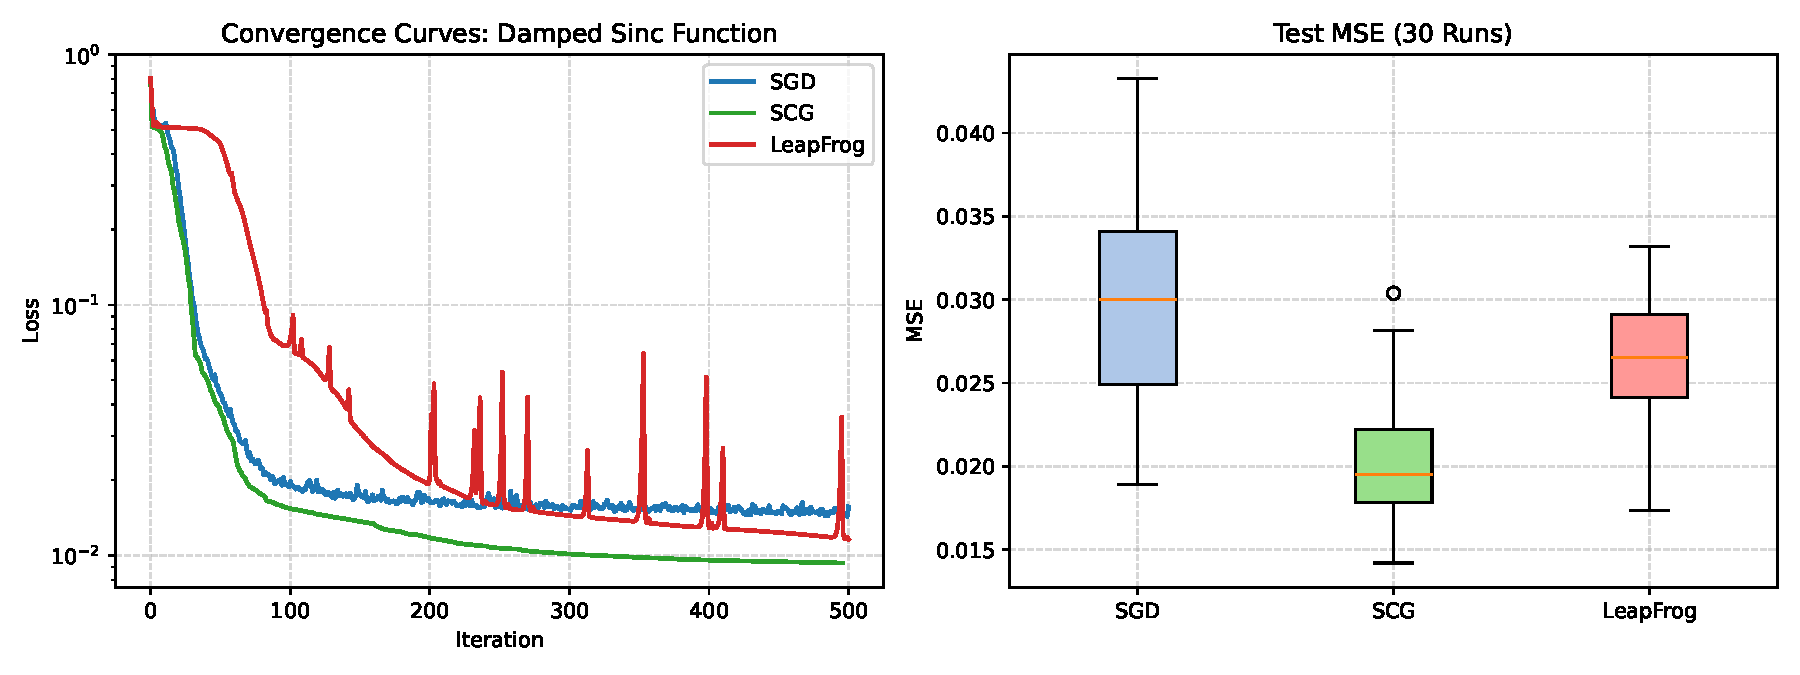
\includegraphics[width=0.32\textwidth]{../results/figures/regression_1_comparison.pdf}
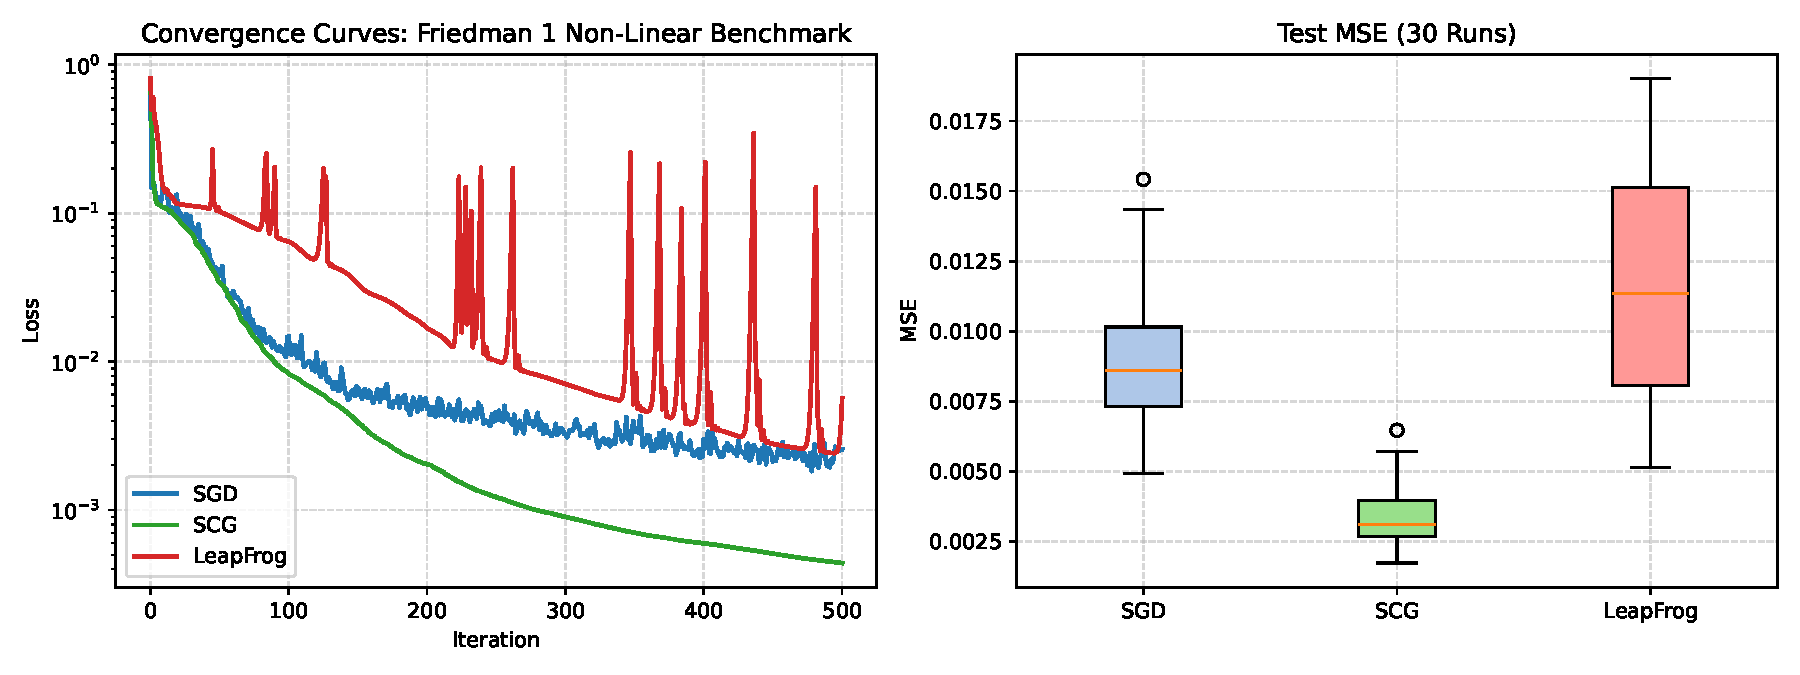
\includegraphics[width=0.32\textwidth]{../results/figures/regression_2_comparison.pdf}
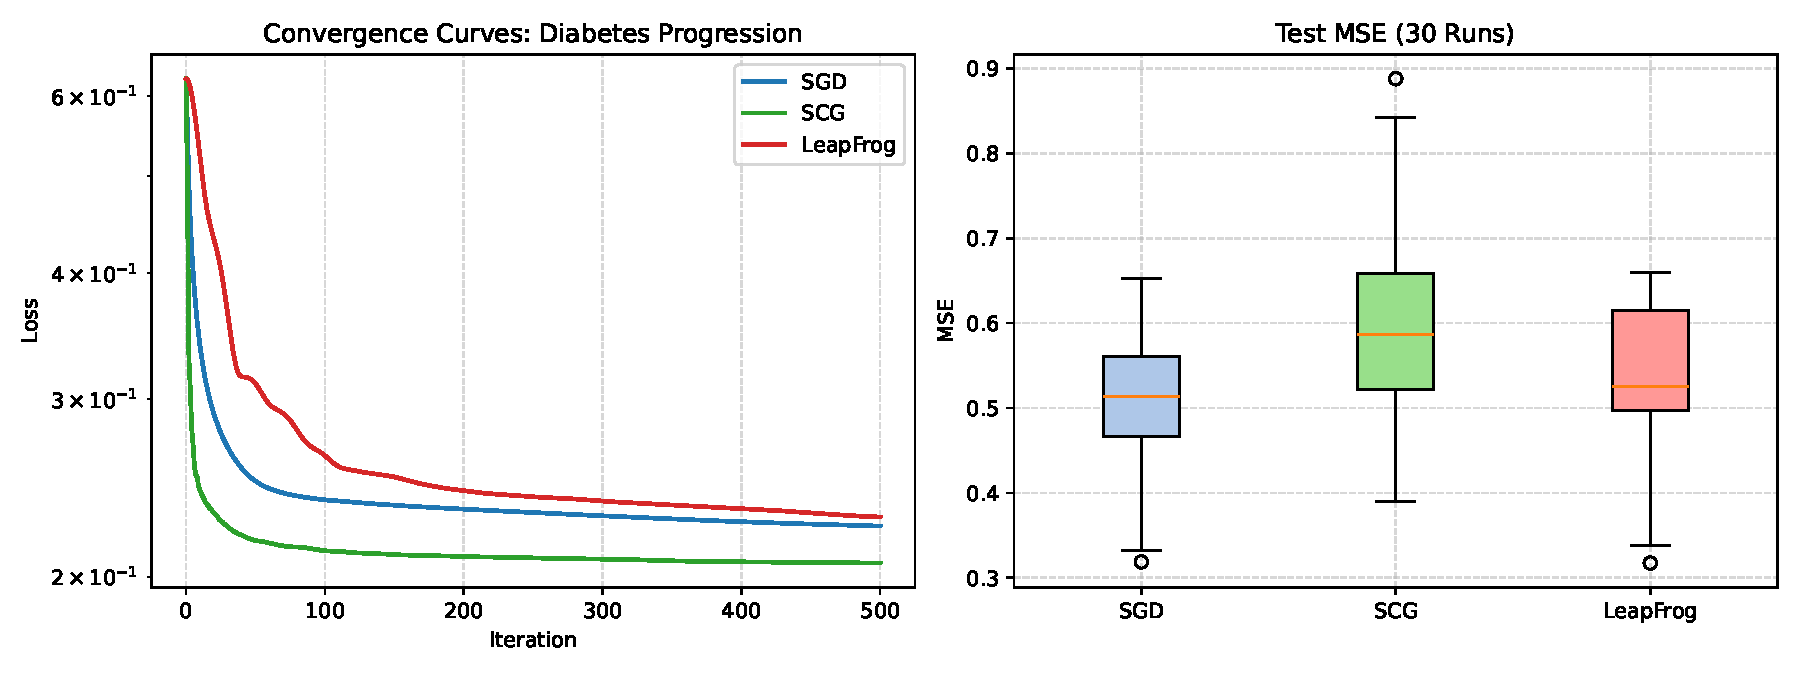
\includegraphics[width=0.32\textwidth]{../results/figures/regression_3_comparison.pdf}
\caption{Convergence trajectories and performance distributions across regression benchmarks.}
\label{fig:reg_curves}
\end{figure*}

\subsection{Computational Efficiency and Convergence Dynamics}
Figure \ref{fig:class_curves} and Figure \ref{fig:reg_curves} illustrate the convergence trajectories and error distributions across the classification and regression problems, respectively.

Inspection of function and gradient evaluation counts in Table \ref{tab:comparison} highlights the contrasting computational profiles of the methods. Stochastic gradient descent required between 2000 and 7000 gradient evaluations per run due to mini-batch parameter updates across iterations. In contrast, the leap-frog dynamic optimizer executed exactly 501 gradient evaluations per run, corresponding to one gradient evaluation per time step. Scaled conjugate gradient executed between 815 and 1000 gradient evaluations, utilizing two gradient evaluations per accepted step to estimate directional second-order information.

In terms of wall-clock execution time, leap-frog was consistently the fastest training algorithm across all datasets, requiring an average of 0.074 to 0.287 seconds per training run. Scaled conjugate gradient ranked second in computational speed, averaging 0.096 to 0.452 seconds. Stochastic gradient descent exhibited the highest computational cost, averaging 0.159 to 0.722 seconds, driven by repetitive memory access and backward passes over mini-batches.

\section{Conclusions}
This study evaluated three feedforward neural network training algorithms: stochastic gradient descent, scaled conjugate gradient, and the leap-frog dynamic optimizer. Empirical evaluations across three classification problems and three function approximation problems revealed distinct performance characteristics. The scaled conjugate gradient algorithm achieved the highest accuracy and lowest generalization error on non-linear function approximation and continuous manifold classification tasks, converging within fewer iterations than stochastic gradient descent. Stochastic gradient descent demonstrated robust performance on noisy clinical regression and diagnostic datasets, but incurred the highest computational execution time and largest number of gradient evaluations. The leap-frog dynamic optimization method demonstrated the lowest computational complexity per iteration and required the fewest gradient evaluations while achieving competitive accuracy across all benchmarks.

\begin{thebibliography}{00}

\bibitem{moller1993}
M.~F.~M\o{}ller, ``A scaled conjugate gradient algorithm for fast supervised learning,'' \emph{Neural Networks}, vol.~6, no.~4, pp.~525--533, 1993.

\bibitem{polyak1964}
B.~T.~Polyak, ``Some methods of speeding up the convergence of iteration methods,'' \emph{USSR Computational Mathematics and Mathematical Physics}, vol.~4, no.~5, pp.~1--17, 1964.

\bibitem{snyman1982}
J.~A.~Snyman, ``A new and dynamic method for unconstrained minimization,'' \emph{Applied Mathematical Modelling}, vol.~6, no.~6, pp.~449--462, 1982.

\bibitem{snyman1983}
J.~A.~Snyman, ``An improved version of the original leap-frog dynamic method for unconstrained minimization: LFOP1(b),'' \emph{Applied Mathematical Modelling}, vol.~7, no.~3, pp.~216--218, 1983.

\end{thebibliography}

\appendices

\section{Acronyms}
\begin{itemize}
    \item \textbf{LFOP1}: Leap-frog optimizer version 1
    \item \textbf{LFOP1(b)}: Leap-frog optimizer version 1 (modified)
    \item \textbf{MSE}: Mean squared error
    \item \textbf{SCG}: Scaled conjugate gradient
    \item \textbf{SD}: Standard deviation
    \item \textbf{SGD}: Stochastic gradient descent
\end{itemize}

\section{Mathematical Symbols}
\begin{itemize}
    \item $\mathbf{a}_k$: Acceleration vector at step $k$
    \item $\alpha_k$: Step size parameter in scaled conjugate gradient
    \item $\mathbf{b}^{(l)}$: Bias vector of layer $l$
    \item $\beta$: Momentum coefficient
    \item $D$: Parameter space dimensionality
    \item $\delta$: Maximum allowable displacement in leap-frog
    \item $\delta_k$: Quadratic curvature parameter in scaled conjugate gradient
    \item $\Delta_k$: Model comparison parameter in scaled conjugate gradient
    \item $\Delta t$: Discretization time step in leap-frog
    \item $\eta$: Learning rate parameter
    \item $E(\mathbf{w})$: Scalar objective error function
    \item $\mathbf{p}_k$: Conjugate search direction vector at step $k$
    \item $\mathbf{s}_k$: Estimated Hessian-vector product vector
    \item $\sigma$: Finite-difference perturbation scalar in scaled conjugate gradient
    \item $\mathbf{v}_k$: Velocity vector at step $k$
    \item $\mathbf{w}_k$: Concatenated parameter vector at step $k$
    \item $\mathbf{W}^{(l)}$: Weight matrix of layer $l$
    \item $\mathbf{x}$: Input feature vector
    \item $\mathbf{y}$: Target output vector
    \item $\hat{\mathbf{y}}$: Model predicted output vector
\end{itemize}

\end{document}
